\newcommand{\grad}{$^{\circ}$}
\capitulo{1}{Introducción}
%\maketitle
Este proyecto es un trabajo que se hará en colaboración con el Laboratorio de Evolucion Humana \footnote{ \url{http://www3.ubu.es/atapuerca/index.html}}, del departamento de Ciencias Históricas de la Universidad de Burgos. Concretamente, la colaboradora del proyecto será la Dra. Rebeca García González \cite{ubu:Rebe},  que estudia paleobiología y paleoecología de homínidos en la Universidad de Burgos. 

El problema planteado, que se quiere automatizar, consiste en crear una herramienta o aplicación para detectar las estrías que se producen en los dientes al masticar distintos tipos de comida, tal y como se explica en el artículo en el que nos basaremos para desarrollar el método \cite{garcia2015dietary}.

La dureza de los distintos materiales es tangible. Concretamente, los dientes tienen una dureza superior a la de los alimentos, sin embargo algunas partes de los alimentos tienen mas dureza que los dientes, por lo que los consiguen rallar, creando unas estrías que dependiendo de los alimentos siguen distintos patrones.

 
Con este método de trabajo vamos a detectar esas estrías, pero en el contexto de la prehistoria, para después poder clasificar los individuos en función de la dieta que llevaban. La forma de clasificacion en las direcciones esta determinada por el artículo \cite{garcia2015dietary}, en el que nos indican los ángulos de clasificación para las 4 direcciones:
\begin{itemize}
\item Horizontales <<H>>: Con ángulos comprendidos de 0\grad - 22.5\grad y de 157.5\grad - 180\grad.
\item Verticales <<V>>: Con ángulos comprendidos de 67.5\grad - 112.5\grad. 
\item Disto-occlusal a mesio-cervical <<DM>>: Con ángulos comprendidos de 112.5\grad - 157.5\grad.
\item Mesio-occlusal a disto-cervical <<MD>>: Con ángulos comprendidos de 22.5\grad - 67.5\grad.
\end{itemize}
Para mas tarde extrapolar los datos de estas orientaciones y proyectar un punto en un plano de dos dimensiones, que nos indicara a que región pertenece dicho individuo y esto podrá ser estimado por las dos funciones que propone Lalueza en su artículo \cite{Lalueza:perez}. 

Los tipos de dieta son los sigientes: 
\begin{itemize}
\item Agricultores.
\item Cazadores recolectores de climas áridos.
\item Cazadores recolectores de climas tropicales.
\item Cazadores carnívoros.
\end{itemize}
Para ver como seria la clasificacion en elarticulo añadiremso la captura de la grafica que detalla el artículo de Rebeca García \ref{fig:clasiDieta}

\begin{figure}[h]
\centering
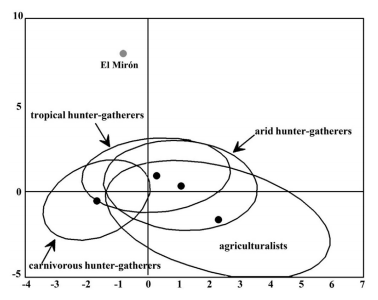
\includegraphics[width=.65\textwidth]{clasiDieta}
\caption{Clasificación en dietas usada por Rebeca Garcia en~\cite{garcia2015dietary}.}
\label{fig:clasiDieta}
\end{figure}


Nuestro proyecto va a tener una parte de visión artificial, que detecte las lineas que han pintado sobre las imágenes de microscopio de electrones a 100 aumentos. Otra parte de diseño e implementación del software a usar y distintos análisis de las herramientas que usaremos para ello.

La herramienta a usar tendrá implementados 3 modos claramente diferenciados.

\begin{itemize}
\item Modo semi-automático: detección, conteo y análisis de las lineas pintadas sobre una imagen.
\item Pintar lineas manualmente sobre la imagen o corregir las posibles lineas que el anterior modo no consiga detectar.
\item Automático que buscará las estrías por la imagen. Este modo quedará como extra, ya que hemos tenido una gran agilidad realizando el proyecto, vamos a tratar esta parte para completar e investigar sobre detección automática de bordes.
\end{itemize}








 